
% --- SLIDE 1 : Context Image ---
\begin{frame}{Introduction: Flow Matching Context}
    \centering
    % Make sure 'schema_flow_matching.png' is uploaded to your project
    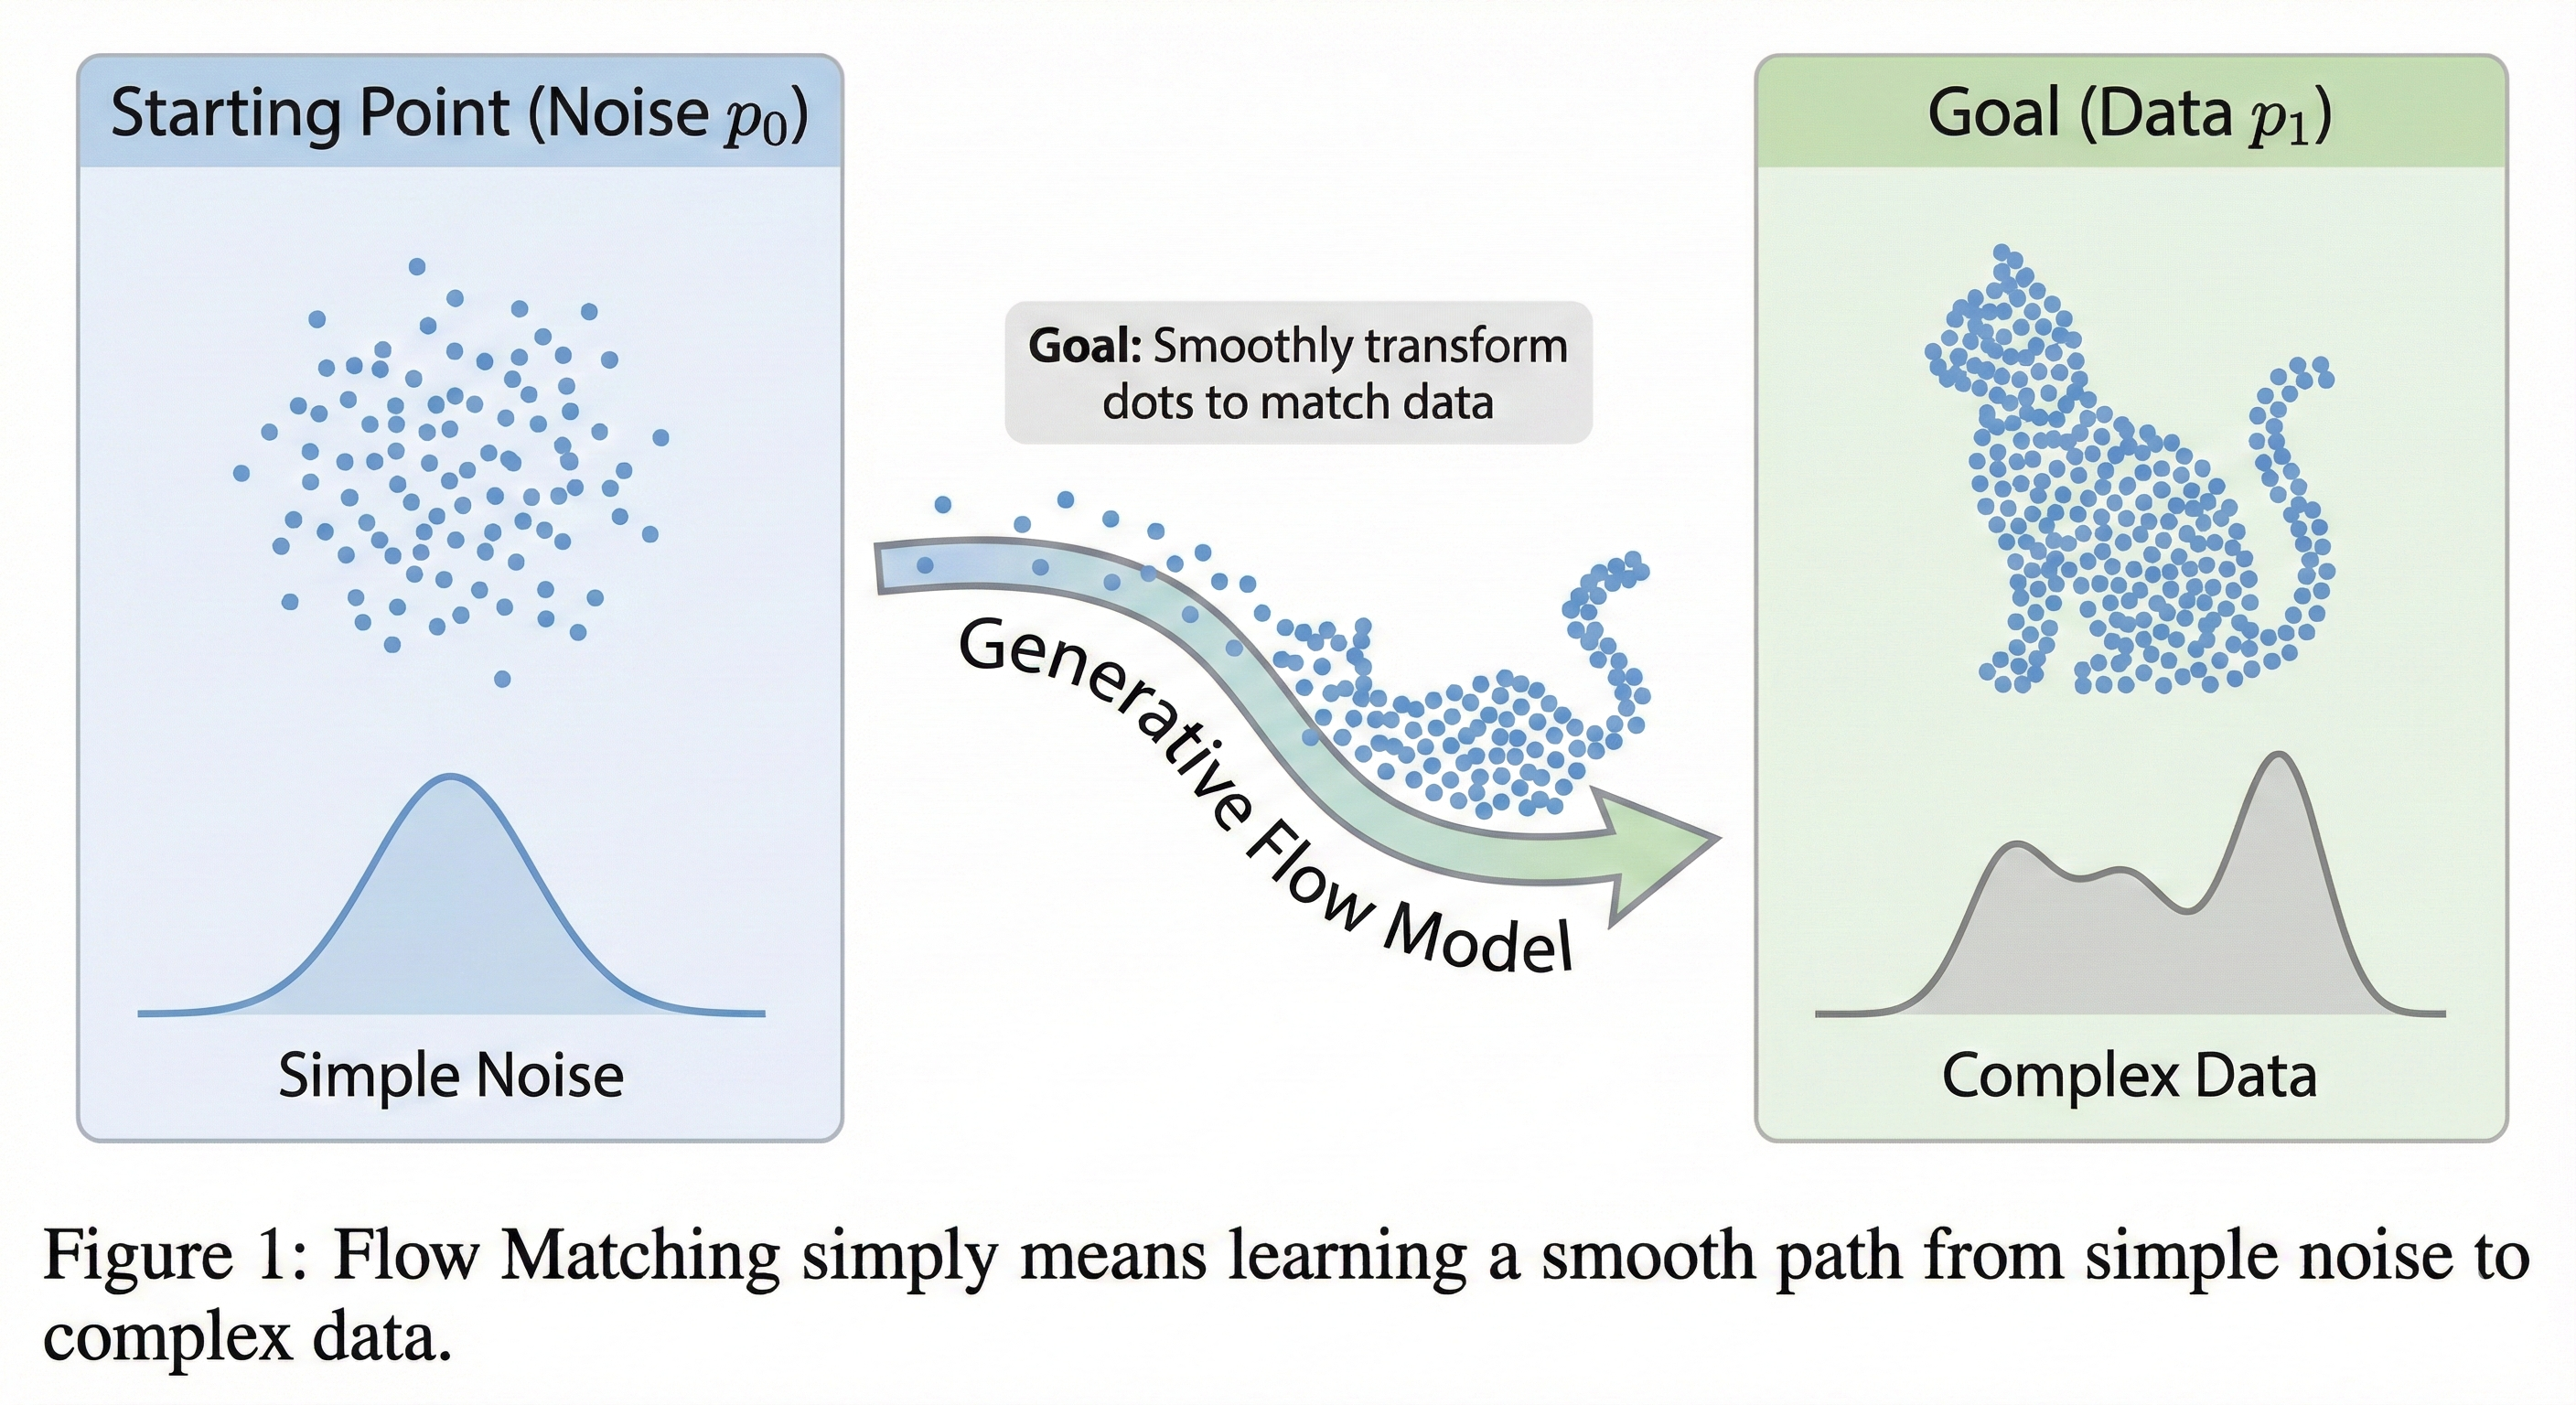
\includegraphics[width=0.9\textwidth]{imgs/schema_flow_matching.png}
\end{frame}

% --- SLIDE 2 : Introduction Formelle ---
\begin{frame}{The Transport Problem}
    \begin{block}{Objective: Generative Modeling}
        Let $p_0$ be a source distribution (Gaussian noise) and $p_1$ an unknown target distribution (data).
        We seek a \textbf{diffeomorphism} $\phi : \R^d \to \R^d$ such that:
        $$ \phi_* p_0 = p_1 \quad (\text{Push-forward}) $$
    \end{block}

    \vspace{0.5cm}

    \begin{columns}
        \column{0.6\textwidth}
        \textbf{Our Approach: Optimal Transport Path}
        \begin{itemize}
            \item We define the probability path $p_t$ via linear interpolation.
            \item Stochastic Process:
            $$ \mathbf{x}_t = (1-t)\mathbf{x}_0 + t\mathbf{x}_1 $$
        \end{itemize}

        \column{0.4\textwidth}
        \centering
        % Vector Schematic
        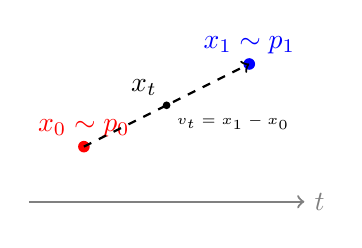
\begin{tikzpicture}[scale=0.7]
            \draw[->, thick, gray] (-1,0) -- (4,0) node[right] {$t$};
            % Points
            \fill[red] (0,1) circle (3pt) node[above] {$x_0 \sim p_0$};
            \fill[blue] (3,2.5) circle (3pt) node[above] {$x_1 \sim p_1$};
            % Trajectory
            \draw[->, thick, dashed] (0,1) -- (3,2.5) node[midway, below right, font=\tiny] {$v_t = x_1 - x_0$};
            \fill[black] (1.5, 1.75) circle (2pt) node[above left] {$x_t$};
        \end{tikzpicture}
    \end{columns}
\end{frame}

% --- SLIDE 3 : The Jacobian Problem ---
\begin{frame}{Baseline: Normalizing Flows and the Jacobian Bottleneck}
    The discret flow of RealNVP is a finished series of steps. The model is defined as an integer number of layers :
$$x_0 \rightarrow x_1 \rightarrow x_2 \rightarrow ... \rightarrow x_k$$
$$z = f_k(...f_2(f_1(x)))$$


    Let $f_\theta : \mathcal{X} \to \mathcal{Z}$ be an invertible generative model.
    According to the \textbf{Change of Variable Theorem}, the log-likelihood is:

    \begin{equation*}
        \log p_X(x) = \log p_Z(f_\theta(x)) + \log \left| \det \left( \frac{\partial f_\theta(x)}{\partial x} \right) \right|
    \end{equation*}

\end{frame}

% --- SLIDE 5 : RealNVP Simplified Math ---
\begin{frame}{RealNVP: The Affine Coupling Trick}
    We splits the data into two parts $(x_a, x_b)$.
    
    \vspace{0.3cm}
    \textbf{The Strategy:}

    $$
    \begin{cases}
        y_a = x_a & (\text{Identity}) \\
        y_b = x_b \cdot \exp(s(x_a)) + t(x_a) & (\text{Affine Transform})
    \end{cases}
    $$

    \centering 
    \includegraphics[width=0.5\textwidth]{imgs/real_nvp_schema.png}
\end{frame}